\documentclass[14pt, a4paper]{extarticle}

\usepackage{my_GOST}
\usepackage{hyperref}
\usepackage{listings}
\usepackage{array}
\usepackage{caption}
\hypersetup{
	pdftex,
	colorlinks = true,
	linkcolor = black,
	filecolor = magenta,
	citecolor = green,      
	urlcolor = cyan,
}

% к таблице и листингу подпись сверху, перед каждым иллюстративным материалом анонсировать
% написатьт в квадратных скобках к рекурсии комментарием что это метод и понятно почему вызываем его снова
\definecolor{mylightgray}{RGB}{240,240,240}
\definecolor{mygreen}{rgb}{0,0.6,0}
\definecolor{mygray}{rgb}{0.5,0.5,0.5}
\definecolor{mymauve}{rgb}{0.58,0,0.82}

\lstset{
	backgroundcolor=\color{mylightgray},rulecolor=\color{red},  % choose the background color; you must add \usepackage{color} or \usepackage{xcolor}; should come as last argument
	basicstyle=\footnotesize\ttfamily,        % the size of the fonts that are used for the code
	breakatwhitespace=false,         % sets if automatic breaks should only happen at whitespace
	breaklines=true,                 % sets automatic line breaking
	captionpos=t,                    % sets the caption-position to bottom
	commentstyle=\color{mygreen},    % comment style
	extendedchars=false,              % lets you use non-ASCII characters; for 8-bits encodings only, does not work with UTF-8
	firstnumber=0,                % start line enumeration with line 1000
	frame=shadowbox,
	%rulesepcolor=\color{green},	                   % adds a frame around the code
	keepspaces=true,                 % keeps spaces in text, useful for keeping indentation of code (possibly needs columns=flexible)
	keywordstyle=\color{blue}\textbf,       % keyword style
	language=C++,                 % the language of the code
	morekeywords={*,...},            % if you want to add more keywords to the set
	numbers=left,                    % where to put the line-numbers; possible values are (none, left, right)
	numbersep=5pt,                   % how far the line-numbers are from the code
	numberstyle=\scriptsize\color{mygray}, % the style that is used for the line-numbers
	rulecolor=\color{black},         % if not set, the frame-color may be changed on line-breaks within not-black text (e.g. comments (green here))
	showspaces=false,                % show spaces everywhere adding particular underscores; it overrides 'showstringspaces'
	showstringspaces=false,          % underline spaces within strings only
	showtabs=false,                  % show tabs within strings adding particular underscores
	stepnumber=1,                    % the step between two line-numbers. If it's 1, each line will be numbered
	stringstyle=\color{mymauve},     % string literal style
	tabsize=4,	                   % sets default tabsize to 2 spaces
	title=\lstname                   % show the filename of files included with \lstinputlisting; also try caption instead of title
}
\usepackage{YATPR}

\usepackage[utf8]{inputenc}
\usepackage{amsmath}
\usepackage{float}

\begin{document}
\begin{titlepage}
	\newgeometry{pdftex, left=2cm, right=2cm, top=2.5cm, bottom=2.5cm}
	\fontsize{12pt}{12pt}\selectfont
	\noindent \begin{minipage}{0.15\textwidth}
		
\includegraphics[width=\linewidth]{pictures/b_logo.jpg}
	\end{minipage}
	\noindent\begin{minipage}{0.9\textwidth}\centering
		\textbf{Министерство науки и высшего образования Российской Федерации}\\
		\textbf{Федеральное государственное бюджетное образовательное учреждение высшего образования}\\
		\textbf{«Московский государственный технический университет имени Н.Э.~Баумана}\\
		\textbf{(национальный исследовательский университет)»}\\
		\textbf{(МГТУ им. Н.Э.~Баумана)}
	\end{minipage}
	
	\noindent\rule{18cm}{3pt}
	\newline\newline
	\noindent ФАКУЛЬТЕТ $\underline{\text{«Информатика и системы управления»}}$ \newline\newline
	\noindent КАФЕДРА $\underline{\text{«Программное обеспечение ЭВМ и информационные технологии»}}$\newline\newline\newline\newline\newline\newline\newline
	
	
	\begin{center}
		\Large\textbf{Отчет по лабораторной работе №5}\newline
	\end{center}
	
	\noindent\textbf{Название} $\underline{\text{~Моделирование работы информационного центра~~~~~~~~~}}$\newline\newline\newline
	\noindent\textbf{Дисциплина} $\underline{\text{~Моделирование~~~~~~~~}}$\newline\newline
	\noindent\textbf{Студент} $\underline{\text{Зайцева А. А.~~~~~~~~~~~~~~~~~~~~~~~~~~~~~~~~~~~~~~~~~}}$\newline\newline
	\noindent\textbf{Группа} $\underline{\text{ИУ7-72Б~~~~~~~~~~~~~~~~~~~~~~~~~~~~~~~~~~~~~~~~~~~~}}$\newline\newline
	\noindent\textbf{Оценка (баллы)} $\underline{\text{~~~~~~~~~~~~~~~~~~~~~~~~~~~~~~~~~~~~~~~~~~~~~~~~~}}$\newline\newline
	\noindent\textbf{Преподаватель}$\underline{\text{~Рудаков И. В.~~~~~~~~~~}}$\newline
	
	\begin{center}
		\vfill
		Москва~---~\the\year
		~г.
	\end{center}
 \restoregeometry
\end{titlepage}


\setcounter{page}{2}

\section{Задание}



Дана концептуальная модель парковки торгового центра, где также предоставляется услуга автомойки: 
\begin{itemize}
	\item количество мест на парковке $\textit{parking\_spaces}=50$;
	\item количество мест для автомойки $\textit{n\_washers}=5$;
	
	\item количество новых клиентов, которые приезжают на парковку каждую минуту, распределенно по закону Пуассона с параметром \\$\textit{requests\_lambda}=3$;
	\item вероятность того, что владелец обратится за услугой мойки автомобиля $\textit{washing\_p}=0.1$;
	\item клиент, в зависимости от того, требуется ему услуга мойки или нет, встает в очередь либо к оператору автомойки, либо к оператору парковки;

	\item если клиент встал в очередь к оператору парковки, а длина этой очереди больше $\textit{max\_operator\_parking\_len}=30$, то клиент расстраивается и уезжает, иначе ожидает в очереди;
	\item оператор парковки может начать печатать талон для текущего клиента, только если на парковке есть свободное место, оператор парковки обрабатывает одного клиента за $2\pm1$ минуту;
	
	\item если клиент встал в очередь к оператору мойки, и длина этой очереди больше $\textit{max\_operator\_washing\_len}=5$, то клиент расстраивается и уезжает, иначе ожидает в очереди;
	\item оператор мойки может начать печатать талон для текущего клиента, если есть свободное место на автомойке (тогда клиент сразу отправляется на автомойку) или если есть свободное место на парковке (тогда клиент занимает место на парковке и ставится в очередь на автомойку), оператор автомойки обрабатывает одного клиента за $2\pm1$ минуту;
	

	\item мойка одного автомобиля занимает $60\pm20$ минут;
	\item если клиенту не требуется автомойка, значит он идет в торговый центр и проводит там время, распределенное по нормальному закону с параметрами $m=150$ минут и $\sigma=10$;
		

	\item когда услуга автомойки завершена или клиент вернулся из торгового центра, клиент освобождает парковочное место и встает в очередь к оператору оплаты, оператор оплаты обрабатывает одного клиента за $3\pm1$ минуту;
	
\end{itemize}

За единицу имитационного времени принять 0.01 минуты.

Промоделировать процесс обработки 10000 клиентов. Определить имитационное время моделирования; процент клиентов, которым потребовалась услуга автомойки; проценты клиентов, которые отказались от услуг парковки и автомойки; максимальную длину очереди на оплату. Также провести моделирование при изменении отдельных параметров модели.

Построить структурную схему модели, а также схему модели в терминах систем массового обслуживания (СМО).




\section{Теоретическая часть}


В процессе взаимодействия клиентов с парковкой с услугой автомойки возможны два режима работы.
\begin{enumerate}
	\item Режим нормального обслуживания: клиент получает требуемую услугу.
	\item Режим отказа от услуги: если очередь превышает предельно допустимую.
\end{enumerate}


\textbf{Эндогенные переменные}: количество парковочных мест, время обработки клиентов операторами; длины очередей, при которых клиенты отказываются от услуг; время, которое клиенты проводят в торговом центре; время мойки автомобиля.

\textbf{Экзогенные переменные}: $p_0$ -- число клиентов, которые припарковались и сходили в торговый центр, $p_1$ -- число  клиентов, которые решили не дожидаться освобождения мест для парковки; $w_0$ -- число клиентов, которые получили услугу автомойки, $w_1$ -- число  клиентов, которые решили не дожидаться освобождения мест для автомойки.

\textbf{Уравнения модели:} 
\begin{itemize}
	\item процент клиентов, которым потребовалась услуга автомойки:
	\begin{equation}
		w = \frac{w_0 + w_1}{p_0 + p_1 + w_0 + w_1} \cdot 100\%;
	\end{equation}

	\item процент клиентов, которые отказались от услуги парковки:
\begin{equation}
	p_{\textit{p}} = \frac{p_1}{p_0 + p_1} \cdot 100\%;
\end{equation}

	\item процент клиентов, которые отказались от услуги автомойки:
\begin{equation}
	p_{\textit{w}} = \frac{w_1}{w_0 + w_1} \cdot 100\%;
\end{equation}
\end{itemize}


\clearpage
Структурная схема модели приведена на рисунке~\ref{pic:01}.
\begin{figure}[h]
	\begin{center}
		{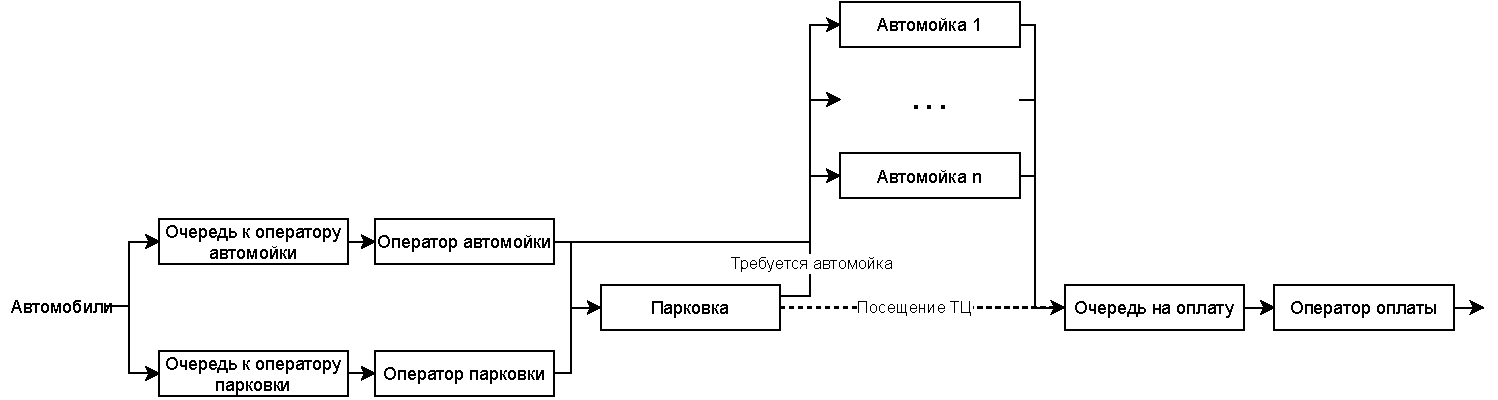
\includegraphics[scale=0.7]{pictures/2-1.pdf}
			\caption{Структурная схема модели}
			\label{pic:01}}
	\end{center}
\end{figure}


Схема модели в терминах СМО приведена на рисунке~\ref{pic:02}.
\begin{figure}[h]
	\begin{center}
		{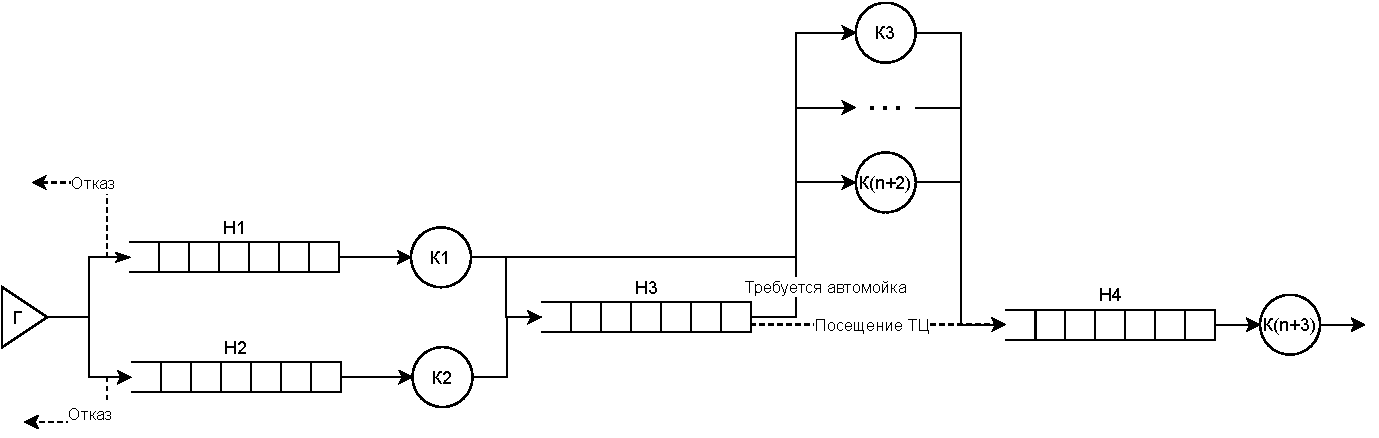
\includegraphics[scale=0.7]{pictures/2-2.pdf}
			\caption{Схема модели в терминах СМО}
			\label{pic:02}}
	\end{center}
\end{figure}

\section{Результаты работы программы}

Для исследования разработанная программа была протестирована при различных: количестве генерируемых клиентов; параметре $\lambda$ распределения Пуассона, по которому распределено количество новых клиентов в минуту; количестве мест для мойки автомобиля; вероятности того, что клиент обратится за услугой автомойки; количестве мест на парковке. На рисунке \ref{pic:res} приведена таблица, где описаны параметры и результаты моделирования. В каждом случае изменялось не более одного (указанного в таблице) параметра, остальные сохранялись из условия. 

\begin{figure}[h]
	\begin{center}
		{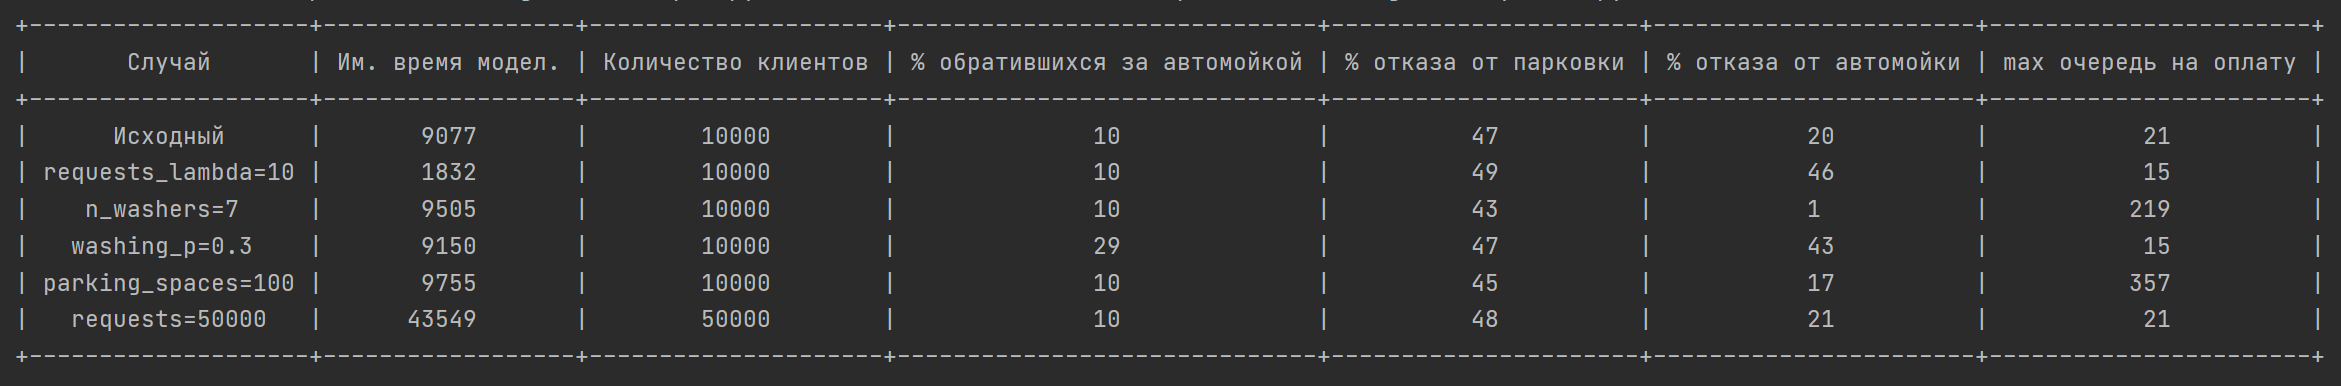
\includegraphics[scale=0.5]{pictures/res.png}
			\caption{Таблица с результатами исследования программы}
			\label{pic:res}}
	\end{center}
\end{figure}



\section{Код программы}

В листинге \ref{lst:list1} приведен код разработанной программы (используемый язык -- Python). 

\begin{lstlisting}[caption = {Код разработанной программы}, label=lst:list1]
from typing import *
from prettytable import PrettyTable
from random import random, seed
from scipy.stats import poisson
from numpy.random import normal
seed(1)

MOD_TIME_STEP = 0.01


class UniformlyDistributedTimeGenerator:
	def __init__(self, a: float, b: float):
		self.a = a
		self.b = b
	
	def generate(self):
		return self.a + (self.b - self.a) * random()


class NormallyDistributedTimeGenerator:
	def __init__(self, m: float, sigma: float):
		self.m = m
		self.sigma = sigma
	
	def generate(self):
		return normal(self.m, self.sigma)


class PoissonDistributedTimeGenerator:
	def __init__(self, lambda_value: int):
		self.lambda_value = lambda_value
	
	def generate(self):
		return poisson.rvs(self.lambda_value, size=1)[0]


class Request:
	def __init__(self, washing_p):
		self.need_wash = random() < washing_p


class RequestsGenerator:
	def __init__(self, time_generator, washing_p):
		self.remaining_time = 0
		self.time_generator = time_generator
		self.washing_p = washing_p
	
	def update_time_and_check_for_request(self):
		if self.remaining_time > 0:
			self.remaining_time -= MOD_TIME_STEP
			return None
		else:
			t = self.time_generator.generate()
			if t == 0:
				self.remaining_time = 1
			else:
				self.remaining_time = 1 / t
			return Request(self.washing_p)


class OnePlaceChannel:
	def __init__(self, accum_in: List, accum_out: List, time_generator, max_out_accum=None):
		self.accum_in = accum_in
		self.accum_out = accum_out
		self.time_generator = time_generator
		self.max_out_accum = max_out_accum
		
		self.is_busy = False
		self.remaining_time = 0
		self.processed_count = 0
	
	def update_time(self):
		processed = False
		if self.max_out_accum is None or len(self.accum_out) < self.max_out_accum:
			if self.is_busy:
				self.remaining_time -= MOD_TIME_STEP
				
				if self.remaining_time <= 0:
					self.processed_count += 1
					self.is_busy = False
					self.accum_out.append(0)
					processed = True
			
			if not self.is_busy:
				if len(self.accum_in) > 0:
					self.accum_in.pop(0)
					self.is_busy = True
					self.remaining_time = self.time_generator.generate()
		return processed


class SimultaneousChannel:
	def __init__(self, accum_out, time_generator):
		self.accum_in = []
		self.accum_out = accum_out
		self.time_generator = time_generator
		self.processed_count = 0
	
	def start_process_new_request(self):
		self.accum_in.append(self.time_generator.generate())
	
	def update_time(self):
		left_times = []
		finished_count = 0
		for time in self.accum_in:
			time -= MOD_TIME_STEP
			if time > 0:
				left_times.append(time)
			else:
				finished_count += 1
				self.accum_out.append(0)
		self.accum_in = left_times
		self.processed_count += finished_count
		
		return finished_count


def simulate(requests=10000, requests_lambda=1, n_washers=5, washing_p=0.1, parking_spaces=50):
	washing_times = (40, 80)
	tc_m = 150
	tc_sigma = 10
	
	operator_parking_times = [1, 3]
	operator_washing_times = [1, 3]
	operator_paying_times = [2, 4]
	
	max_operator_parking_len = 30
	max_operator_washing_len = 5
	
	operator_parking_accum = []
	operator_washing_accum = []
	washing_accum = []
	parking_accum = []
	paying_accum = []
	processed_accum = []
	
	requests_generator = RequestsGenerator(PoissonDistributedTimeGenerator(lambda_value=requests_lambda), washing_p)
	operator_parking = OnePlaceChannel(operator_parking_accum, parking_accum,
	UniformlyDistributedTimeGenerator(*operator_parking_times), max_out_accum=parking_spaces)
	operator_washing = OnePlaceChannel(operator_washing_accum, parking_accum,
	UniformlyDistributedTimeGenerator(*operator_washing_times), max_out_accum=parking_spaces)
	tc = SimultaneousChannel(paying_accum, NormallyDistributedTimeGenerator(tc_m, tc_sigma))
	washers = [OnePlaceChannel(washing_accum, paying_accum,
	UniformlyDistributedTimeGenerator(*washing_times)) for _ in range(n_washers)]
	operator_paying = OnePlaceChannel(paying_accum, processed_accum,
	UniformlyDistributedTimeGenerator(*operator_paying_times))
	
	washing_generated, parking_generated, washing_rejected, parking_rejected, modeling_time, max_paying_len = 0, 0, 0, 0, 0, 0
	
	while len(processed_accum) < requests:
		if len(paying_accum) > max_paying_len:
			max_paying_len = len(paying_accum)
		
		
		modeling_time += MOD_TIME_STEP
		if (washing_generated + parking_generated) < requests:
			request = requests_generator.update_time_and_check_for_request()
			if request is not None:
				if request.need_wash:
					washing_generated += 1
					if len(operator_washing_accum) >= max_operator_washing_len:
						washing_rejected += 1
						processed_accum.append(0)
					else:
						operator_washing_accum.append(0)
				else:
					parking_generated += 1
					if len(operator_parking_accum) >= max_operator_parking_len:
						parking_rejected += 1
						processed_accum.append(0)
					else:
						operator_parking_accum.append(0)
		
		new_visitor_to_tc = operator_parking.update_time()
		if new_visitor_to_tc:
			tc.start_process_new_request()
		visitors_from_tc = tc.update_time()
		for _ in range(visitors_from_tc):
			parking_accum.pop(0)
		
		washing_request = operator_washing.update_time()
		if washing_request:
			washing_accum.append(0)
		
		for operator in washers:
			washing_finished = operator.update_time()
			if washing_finished:
				parking_accum.pop(0)
		
		operator_paying.update_time()
	

	return washing_generated, parking_generated, washing_rejected, parking_rejected, modeling_time, max_paying_len

def add_row(table, name, washing_generated, parking_generated, washing_rejected, parking_rejected, modeling_time, max_paying_len):
	table.add_row([name, round(modeling_time),
	washing_generated + parking_generated,
	round(100 * washing_generated / (parking_generated + washing_generated)),
	round(100 * parking_rejected / (parking_generated + parking_rejected)),
	round(100 * washing_rejected / (washing_generated + washing_rejected)),
	max_paying_len
	])

def main():
	res_table = PrettyTable()
	res_table.field_names = ['Случай', 'Им. время модел.',
	'Кол-во клиентов', '% обр. за автомойкой',
	'% отказа от парковки', '% отказа от автомойки', 'max очередь на оплату']
	
	add_row(res_table, 'Исходный', *simulate())
	add_row(res_table, 'requests_lambda=10', *simulate(requests_lambda=10))
	add_row(res_table, 'n_washers=7', *simulate(n_washers=7))
	add_row(res_table, 'washing_p=0.3', *simulate(washing_p=0.3))
	add_row(res_table, 'parking_spaces=100', *simulate(parking_spaces=100))
	add_row(res_table, 'requests=50000', *simulate(requests=50000))
	
	print(res_table)


if __name__ == '__main__':
	main()
\end{lstlisting}

\end{document}